The FLAME architecture has some inherently good characteristics that lend itself to parallelisation. Unfortunately, it also has a number of bad characteristics. Because FLAME is an application generator
it does not have a full understanding of the application it is generating. Agent-based applications could be characterised as a set of communicating tasks. Although the agent population and their interactions can be specified \textit{a priori} the computational load of each agent and the number of communications they perform are very difficult to determine without running the code. 

We will not address the dynamic re-configuring of an agent population at run time. Initial experiments have shown that this is a very complex problem where there are many trade offs to be considered. In this effort to have an automatically generated parallel implementation of a FLAME application we focus on the most basic characteristic of FLAME and its agents: that of communications - agent to agent. This communication between agents is implemented within FLAME as a set of \textit{message boards} on which agents post messages (information) and from which agents can read the messages (information). There is one message board per message type and FLAME manages all the users interactions with the message boards through a Message Board API.

In a fully connected and communicating agent population, interaction may not be local but long range leading to many-to-many, inter-node communication which can drastically impact the scalability and simulation time. However, in many applications of FLAME, we have seen that there is sufficient locality (that can be taken advantage of) to consider parallelisation taking into account the general population sizes. 

The use of simple read/write, single-type message boards allows the framework implementer to divide the agent population and their associated communications areas. This division could be based on any number of parameters or separators but the simplest to appreciate is position or locality. If, as in EURACE, agents are people or companies for example, they will have locality defined either as location or by some group topology. It is also reasonable to assume that the dominant communications in both scenarios will be with neighbouring agents.

As explained above, FLAME uses a collection of message boards to facilitate inter-agent communication. As the majority of large high performance computing systems currently use a distributed memory model a Single Program Multiple Data (SPMD) paradigm is considered most appropriate for the FLAME architecture. The parallelisation of FLAME utilises partitioned agent populations and distributed message boards linked through MPI communication. Figure~\ref{fig:Figure2} shows the difference between the serial and parallel implementation.

\begin{figure}[h]
	\centering
		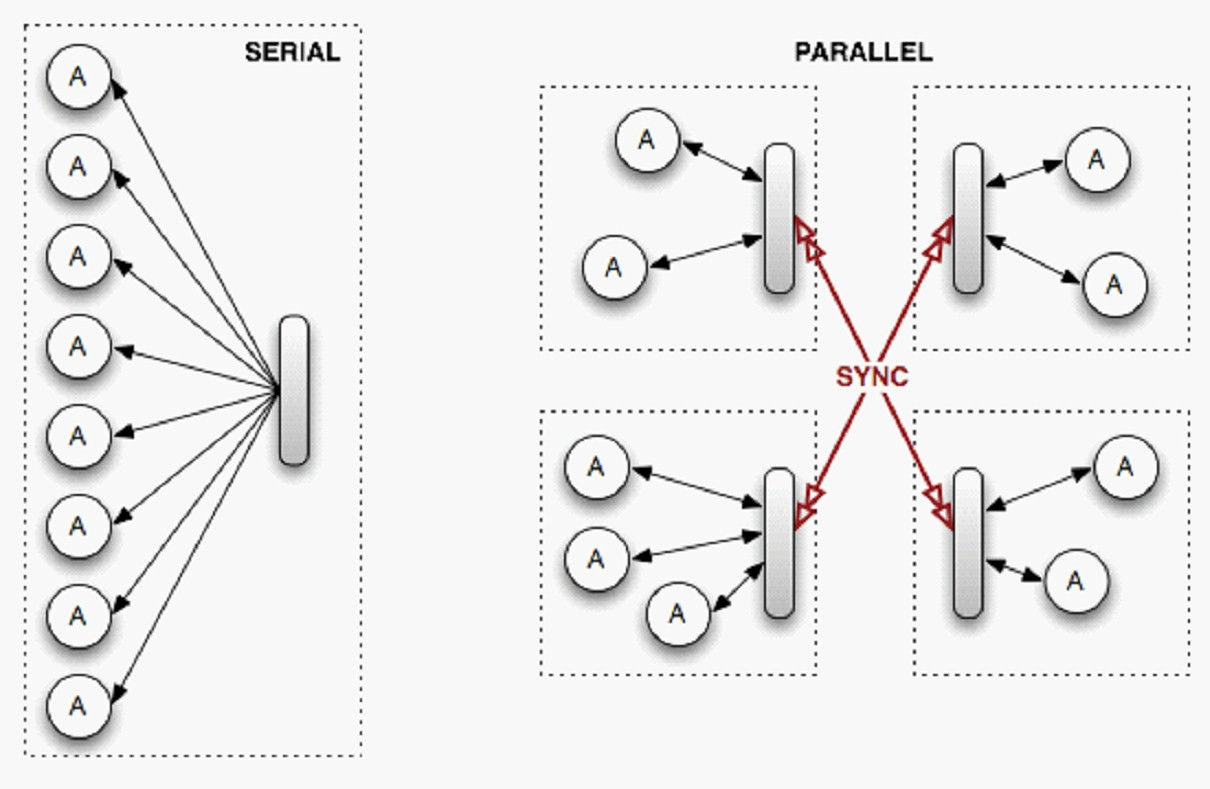
\includegraphics[scale=0.25]{flame.jpg}
	\caption{Serial and Parallel Message Boards}
	\label{fig:Figure2}
\end{figure}

The most significant operation in the parallel implementation is providing the message information required by agents on one node of the processor array but stored on a remote node of the processor. The FLAME Message Board Library manages these data requests by using a set of predefined message filters to limit the message movement. This process could be considered a synchronisation of the local message boards within an iteration of the simulation. This synchronisation essentially ensures that local agents have the message information they need as the simulation progresses.

An additional advantage of implementing parallelism in FLAME through the Message Board Library is that development of the FLAME framework and the message board algorithms can continue independently to a great extend as the Message Board API defines the interface between the two elements of the code. This should enable the message board routines to be developed and optimised without major re-engineering of the framework.

The two main areas of algorithmic and technical development needed to achieve an effective parallel implementation are load balancing and communications strategy. 

Initial load balancing is not too difficult: we have a population of agents, of various complexities, to which we can assign relative weights and so in the most general case the agents can be distributed over the available processors using the weights. This may well give an initial load balance but makes no reference to the possible communication patterns of the agent population. As the simulation develops the numbers of agents in the population may change and adversely affect the load balance of the processors. It is a very interesting and difficult problem to gauge whether the additional work (computation and communication) involved in remedying a load imbalance  is worth the gain. Given that the goal of any dynamic re-organising of the agents is to reduce the elapsed time of the overall simulation, determining whether a process of dynamically re-balancing the population will contribute to this is very problematic. It may well be that a slight load in-balance will have no significant effect of the wall clock time of the simulation. These problems are under investigation.

The patterns and volumes of communication for the population will have a considerable impact on the performance and parallel efficiency of the simulation. In general, agents are rather light-weight in terms of computational load. Where all agents can and do communicate with all others the communications load within and across processors will be great. Fortunately communications within a processor are generally efficient. However across processors this communication can dominate the application. Within FLAME communication between agents is managed by the Message Board Library, which uses MPI to communicate between processors. The Message Board Library implementation attempts to minimise this communication overhead by overlapping the computational load of the agents with the communication. 

Where the agents have some form of locality the initial distribution of agents makes use of this information in placing agents on processing nodes. During the simulation agents can be dynamically re-distributed to maintain computational load balance. However given the light-weight computational nature of many agent types the effect of dynamically re-distributing agents on the grounds of their communications load may well turn out to be more important than considering computational load.

Within the EURACE Project a parallel version of FLAME has been developed using these ideas and the sections below discuss some of the results in performing parallel simulations.

